\documentclass{article}
\usepackage{amsmath}
\usepackage{graphicx}

\renewcommand{\labelenumi}{(\alph{enumi})}
\renewcommand{\labelenumii}{(\roman{enumii})}
\newcommand{\dee}[2]{\frac{\partial{#1}}{\partial{#2}}}
\title{CS181: Clustering and Parameter Estimation}
\author{Danny Zhu \& Tianhui Cai}
\let\b\mathbf

\begin{document}
\maketitle

\section*{Problem 1}
\begin{enumerate}
\item The set of points satisfying the given constraint is an
  $m$-dimensional hypercube of edge $2\epsilon$, so the probability is
  $(2\epsilon)^m$.
\item Then the set of points satisfying the constraint is the
  intersection of a size $2\epsilon$ hypercube centered at $\mathbf x$
  with the unit hypercube; the volume of that set is at most the
  volume of the small hypercube.
\item 
  \begin{align*}
    d(\b x,\b y)^2&=\sum_j(x_j-y_j)^2\\
    d(\b x,\b y)^2&\ge(x_j-y_j)^2\qquad\textrm{for each $j$}\\
    d(\b x,\b y)&\ge|x_j-y_j|\qquad\textrm{for each $j$}\\
    d(\b x,\b y)&\ge\max_j|x_j-y_j|
  \end{align*}
  Now, $d(\b x,\b y)\le\epsilon$ implies $\max_j|x_j-y_j|\le\epsilon$,
  so the set of $\b y$ satisfying the former is a subset of the set
  satisfying the latter; hence the former has a probability of
  occurring that is not greater.
\item We want a probability of at most $\delta$ that no points are
  within $\epsilon$. That probability is 
  $$(1-P(d(\mathbf x,\mathbf y)\leq \epsilon))^n\geq (1-\rho)^n$$
  Setting $(1-\rho)^n=\delta$, it follows that
  $$n\geq \log \delta / \log(1-\rho)$$
\item It does poorly in higher-dimensional spaces because the distance
  between points increases: fixing $\delta$, $\rho$ decreases 
  exponentially with $m$, so that $\log(1-\rho)$ becomes a negative number
  of smaller absolute value, so that the number of points $n$ needed
  for there to be a point $\mathbf y$ within $\epsilon$ of a fixed point  
  $\mathbf x$ increases. 
\end{enumerate}
\section*{Problem 2}
\begin{enumerate}
\item Maximum likelihood: $P(\mathbf X=\mathbf x | \mathbf
  D)=P(\mathbf X = \mathbf x | \Theta=\theta_{ML})$ where
  \[\theta_{ML} = \arg \max_\theta P(\mathbf D|\theta)\]

  MAP: $P(\mathbf X = \mathbf x | \mathbf D) = P(\mathbf X = \mathbf x
  | \Theta = \theta_{MAP})$ where
  \[\theta_{MAP} = \arg \max_\theta P(\mathbf D | \theta)P(\Theta = \theta)\]

  Full Bayes: $P(\mathbf X = \mathbf x | \mathbf D) = \int_\theta P(\mathbf X = \mathbf x | \Theta = \theta)P(\Theta = \theta | \mathbf D)d\theta$

  % ... I just copied these from lecture notes...why is this worth 5 points 
\item $\theta_{MAP}$ maximizes $P(\Theta|\mathbf D)\propto P(\mathbf
  D)=P(\mathbf D | \Theta = \theta)P(\Theta = \theta)$, using Bayes'
  rule, whereas $\theta_{ML}$ does not --- it merely maximizes
  $P(\mathbf D | \Theta = \theta)$ without the $P(\Theta=\theta)$
  factor, i.e. there is no prior. MAP allows us to account for
  situations in which an outcome is unlikely.
  % ...I dunno. 
\item MAP is advantageous over ML because it can take into
  consideration a prior, whereas ML cannot. Priors provide
  regularization, penalizing attributes that are unlikely.  MAP is
  advantageous over full bayes because full bayes requires integration
  steps that can be difficult to perform.
\item
  Consider the following distributions.
  \begin{center}
    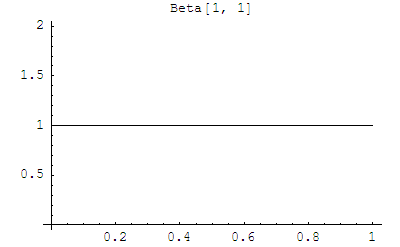
\includegraphics[scale=.35]{beta_1_1.png}
    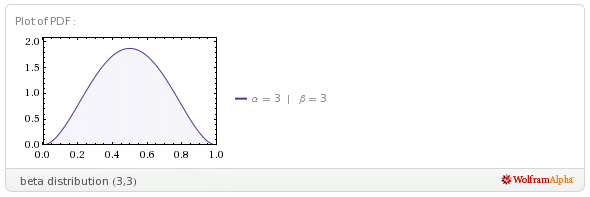
\includegraphics[scale=.35]{beta_3_3.png}
    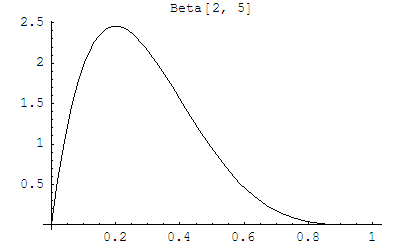
\includegraphics[scale=.35]{beta_2_5.png}
  \end{center}
  A Beta(1,1) is an uninformed prior; it does not give preference to
  any outcome for being more likely. A Beta(3,3) indicates that
  $\theta$ closer to 0.5 is more likely, as it is equivalent to
  assuming that given the data follows a Beta, there were previously 2
  instances classified as 1 and 2 as 0. A Beta(2,5) indicates that
  $\theta$ closer to 0.2 is more likely, as again it is equivalent to
  assuming that given the data follows a Beta, there was one instance
  classifying as 1 and 4 as 0. Outcomes in which $\theta$ is closer to
  1 are penalized for being less likely.
\item The Beta is the conjugate prior of the Bernoulli. In particular,
  $P(\theta | \mathbf D) = \text{Beta} (\Theta = \theta | N_T+\alpha,
  N_F+\beta)$ where the prior is a Beta($\alpha,\beta$). Hence such a
  prior can incorporate information from the prior --- that there were
  previously seen $\alpha-1$ 1's and $\beta-1$ 0's.
\end{enumerate}
\section*{Problem 3}
\begin{enumerate}
\item We require the following parameters.
  \begin{itemize}
  \item 1 for $P(Y)$. Let $\theta_c=P(Y=T)$.
  \item 1 each for $P(X_1|Y=0)$ and $P(X_1|Y=1)$, a total of 2. Let $\theta_1^T=P(X_1=T|Y=T)$. 
  \item 1 each for $P(X_j|X_{j-1},Y)$ for both $Y=0,1$ and $X_{j-1}=0,1$
    over $j=2\ldots m$, so a total of $2\times 2\times (m-1)$. Let $\theta_j^{FT}=P(X_j=T|X_{j-1}=F,Y=T$ and so on. 
  \end{itemize}
  This adds up to $3+4m-4=4m-1$ total parameters.
  % please check this
\item The parameter values are found as follows. First we find log likelihood. 
  \begin{align*}
    \mathcal L(D,\theta) &=
    \sum_{i:y_i=T}\ln \theta_c + \sum_{i:y_i=F}\ln (1-\theta_c) + \\ &
    + \sum_{\stackrel{i:x_{i1}=T}{y_i=T}} \ln \theta_1^T + \sum_{\stackrel{i:x_{i1}=F}{y_i=T}}\ln(1-\theta_1^T)
    + \sum_{\stackrel{i:x_{i1}=T}{y_i=F}} \ln \theta_1^F + \sum_{\stackrel{i:x_{i1}=F}{y_i=F}}\ln(1-\theta_1^F)\\
    &\qquad + \sum_{j=2}^{m} 
    \left[ 
      \sum_{\stackrel{\stackrel{i:x_{ij}=T}{x_{i(j-1)}=T}}{y_i=T}}\ln \theta_{j-1}^{TT} + 
      \sum_{\stackrel{\stackrel{i:x_{ij}=T}{x_{i(j-1)}=F}}{y_i=T}}\ln \theta_{j-1}^{FT} + 
      \sum_{\stackrel{\stackrel{i:x_{ij}=T}{x_{i(j-1)}=T}}{y_i=F}}\ln \theta_{j-1}^{TF} +  \right.\\
      &\qquad\sum_{\stackrel{\stackrel{i:x_{ij}=T}{x_{i(j-1)}=F}}{y_i=F}}\ln \theta_{j-1}^{FF} +  
      \sum_{\stackrel{\stackrel{i:x_{ij}=F}{x_{i(j-1)}=T}}{y_i=T}}\ln (1-\theta_{j-1}^{TT}) + 
      \sum_{\stackrel{\stackrel{i:x_{ij}=F}{x_{i(j-1)}=F}}{y_i=T}}\ln (1-\theta_{j-1}^{FT}) +\\ 
      &\qquad\left.\sum_{\stackrel{\stackrel{i:x_{ij}=F}{x_{i(j-1)}=T}}{y_i=F}}\ln (1-\theta_{j-1}^{TF}) + 
      \sum_{\stackrel{\stackrel{i:x_{ij}=F}{x_{i(j-1)}=F}}{y_i=F}}\ln (1-\theta_{j-1}^{FF})
      \right] \\
  \end{align*}

  Note that all of the paramters have basically the same form. For now
  we find maximum likelihood values for $\theta_c$; the others work the
  same way.  We let $N_{condition}$ denote the number of data points
  that satisfy the condition.
  $$\dee{\mathcal
    L(D,\theta)}{\theta_c}=\frac{N_{Y=T}}{\theta_c}-\frac{N_{Y=F}}{1-\theta_c}$$
  Setting this to 0, we find that
  $$\theta_c=\frac{N_{Y=T}}{N_{Y=F}+N_{Y=T}}$$
  Analogous maximum likelihood values hold for the other parameters. 
  $$\theta_1^T=\frac{N_{X_1=T,Y=T}}{N_{X_1=T,Y=T}+N_{X_1=F,Y=T}}$$
  $$\theta_j^{TF}=\frac{N_{X_j=T,X_{j-1}=T,Y=F}}{N_{X_j=T,X_{j-1}=T,Y=F}+N_{X_j=F,X_{j-1}=T,Y=F}}$$
  ...and so on. 
\item These are pretty similar. Let's do $E[N_{Y=T}]$ for now. 

  $$E[N_{Y=T}]=\sum_i P(Y=T|\mathbf X = \mathbf x_i)$$ Hence it
  suffices to show how to calculate each $P(Y=T|\mathbf X=\mathbf
  x_i)$ using parameter values. By definition,
  \[P(Y=T|\mathbf X = \mathbf x_i)=\frac{P(Y=T, \mathbf X = \mathbf x_i)}{P(\mathbf X = \mathbf x_i)}\]
  so it suffices to show how to calculate the numerator and
  denominator with parameter values. We already know how to calculate
  the numerator: it's the $P(X_1,\ldots,X_m,Y)$ we were given in the
  model, using the parameter values we defined in (a).
  \[P(\mathbf X = \mathbf x_i)=P(\mathbf X = \mathbf x_i, Y=T)P(Y=T)+P(\mathbf X = \mathbf x_i, Y=F)P(Y=F)\]
  Again, we know how to calculate these with parameter
  values. $P(Y=T)$ is $\theta_c$, for instance.

  The other sufficient statistics are calculated analogously, except
  summing over different sets - i.e.,
  \[E[N_{Y=T,\mathrm{condition}}]=\sum_{i, \mathrm{condition}(i)} P(Y=T|\mathbf X=\mathbf x_i)\]
  and
  \[E[N_{Y=N,\mathrm{condition}}]=\sum_{i, \mathrm{condition}(i)} P(Y=N|\mathbf X=\mathbf x_i)\]
  We do this where condition is automatically True, $x_1=T$, $x_1=F$,
  and combinations of $(x_j,x_{j-1})\in \{T,F\}^2$

\item The EM algorithm works entirely analogously to the one given in Lecture 
  11. We'll repeat it anyway.
  \begin{itemize}
  \item Set $\theta_c$, $\theta^T_1$, $\theta^{TT}_j$, $\theta^{TF}_j$, 
    $\theta^{FT}_j$, $\theta^{FF}_j$ to some initial values.
  \item Repeat until convergence:
    \begin{itemize}
    \item Calculate expectations using parameters as in part (c)
    \item Calculate parameters using expectations as in part (b)
    \end{itemize}
  \end{itemize}
  Possibly random-restart to avoid local minima.

\item This model for clustering can be advantageous as it considers interactions
  between different attributes -- specifically, interactions between adjacent
  attributes in a given ordering of the attributes. This is good if the 
  attributes can be ordered to be conditionally independent with the exception 
  of adjacent attributes. Compared to Autoclass, it can realize interactions
  between adjacent attributes, but if there are no interactions between adjacent
  attributes, it can work just as well, i.e. we can just have, say, 
  $\theta_j^{TF}=\theta_j^{FF}$ and so on so that $P(X_j|X_{j-1},Y)=P(X_j|Y)$. 
  We do expect order of attributes matter. ***TODO: example?****
\end{enumerate}
\section*{Problem 4}
\begin{enumerate}
\item 
  \begin{enumerate}
  \item 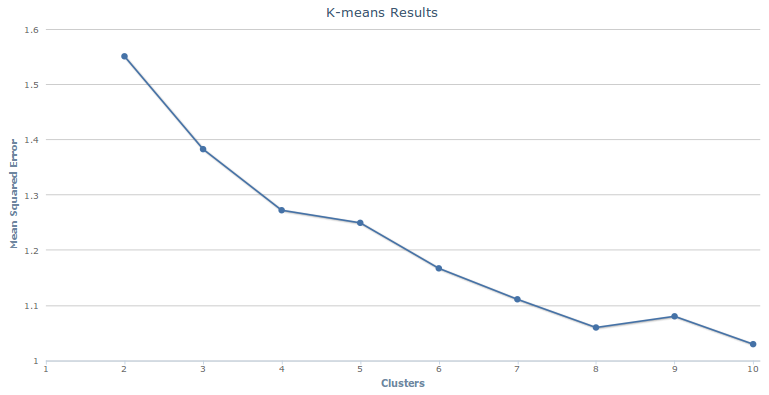
\includegraphics[scale=0.5]{kmeansresults.png} 
  \item We may choose $K=4$ as improvement slows down with
    greater values of $K$. Larger $K$ results in smaller 
    mean squared error, but a smaller $K$ is better for 
    simplicity and so that k-means has fewer iterations. 
  \end{enumerate}
\item 
  \begin{enumerate}
  \item 
  \item 
  \end{enumerate}
\end{enumerate}
\end{document}
